\documentclass{beamer}
\usepackage[utf8]{inputenc}
\usepackage[english]{babel}
\usepackage[T1]{fontenc}
\usepackage[inline]{asymptote}
\usepackage{slide_helper}
\usepackage{asy_helper}
\usepackage{subcaption}
\usepackage{pgfplots}
\pgfplotsset{compat=1.5} 

\title[MATH 1030 - Module 8 - Describing Data]{Describing Data}

\begin{document}
\begin{frame}
\titlepage
\end{frame}

\begin{frame}
\begin{block}{Definition}
A \textbf{frequency table} is a table with two columns. One column lists the categories, and the other the frequencies with which the items in the categories occur. (i.e.\ how many items fit into each category.)
\end{block}\pause

\begin{example}\label{ex:carcolor1}
\begin{columns}[c]
\begin{column}{7cm}
An insurance company determines vehicle insurance premiums based on known risk factors. If a person is considered a higher risk, their premiums will be higher. One potential factor is the color of your car. The insurance company believes that people with some color cars are more likely to get in accidents. 

\vspace{2mm}
To research this, they examined police reports for recent total-loss collisions. The data is summarized in the frequency table.
\end{column}
\begin{column}{3.5cm}
\begin{tabular}{|l|c|}
\hline
\textbf{Color} & \textbf{Frequency} \\\hline
Blue & 25 \\\hline
Green & 52 \\\hline
Red & 41 \\\hline
White & 36 \\\hline
Black & 39 \\\hline
Grey & 23 \\\hline
\end{tabular}
\end{column}
\end{columns}
\end{example}
\end{frame}

\begin{frame}
\begin{block}{Definition}
A \textbf{bar graph} is a graph that displays a bar for each category with the length of each bar indicating the frequency of that category.
\end{block}\pause

\begin{example}
Using the car data from Example~\ref{ex:carcolor1}, we have the following bar graph.

\begin{center}
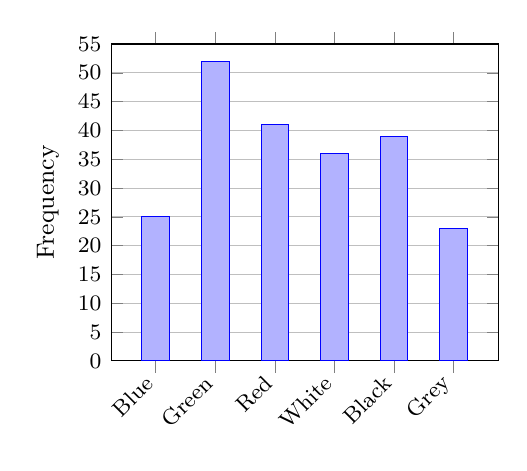
\begin{tikzpicture}
\begin{axis}[
small,
ybar,
enlarge x limits=0.15,
enlarge y limits=false,
legend style={at={(0.5,-0.2)},
anchor=north,legend columns=-1},
ylabel={Frequency},
ymajorgrids=true,
symbolic x coords={Blue, Green, Red, White, Black, Grey},
xtick=data,
x tick label style={rotate=45,anchor=east},
ytick={0,5,...,55},
ymin=0,
ymax=55,
]
\addplot coordinates {
(Blue,25) (Green,52) (Red,41)
(White,36) (Black,39) (Grey, 23)
};
\end{axis}
\end{tikzpicture}
\end{center}
\end{example}
\end{frame}

\begin{frame}
\begin{block}{Definition}
A \textbf{Pareto chart} is a bar graph ordered from highest to lowest frequency.
\end{block}\pause

\begin{example}
Using the car data from Example~\ref{ex:carcolor1}, we have the following Pareto chart.

\begin{center}
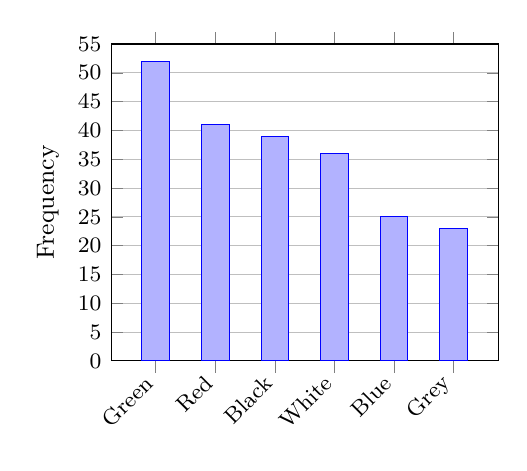
\begin{tikzpicture}
\begin{axis}[
small,
ybar,
enlarge x limits=0.15,
enlarge y limits=false,
legend style={at={(0.5,-0.2)},
anchor=north,legend columns=-1},
ylabel={Frequency},
ymajorgrids=true,
symbolic x coords={Green, Red, Black, White, Blue, Grey},
xtick=data,
x tick label style={rotate=45,anchor=east},
ytick={0,5,...,55},
ymin=0,
ymax=55,
]
\addplot coordinates {
(Blue,25) (Green,52) (Red,41)
(White,36) (Black,39) (Grey, 23)
};
\end{axis}
\end{tikzpicture}
\end{center}
\end{example}
\end{frame}

\begin{frame}
\begin{example}
In a survey\footnote[frame]{Gallup Poll.\ March 5-8, 2009.\ http://www.pollingreport.com/enviro.htm}, adults were asked whether they personally worried about a variety of environmental concerns. The numbers (out of 1012 surveyed) who indicated that they worried \textquote{a great deal} about some selected concerns are summarized below.

\begin{columns}
\begin{column}{0.35\linewidth}
\begin{tabular}{|p{3cm}|c|}
\hline
\textbf{Environmental Issue} & \textbf{Frequency} \\\hline
Water pollution & 597 \\\hline
Toxic waste & 526 \\\hline
Air pollution & 455 \\\hline
Global warming & 354 \\\hline
\end{tabular}
\end{column}
\begin{column}{0.45\linewidth}
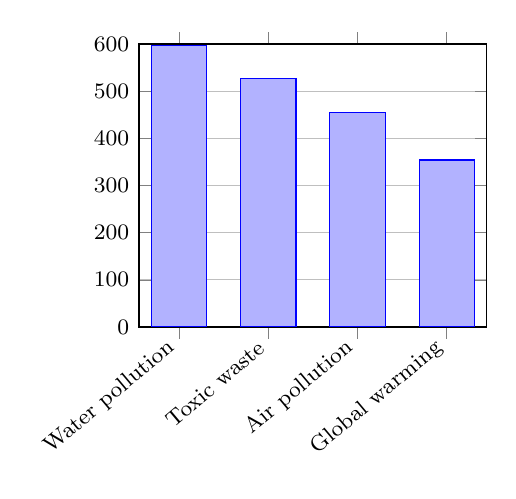
\begin{tikzpicture}
\begin{axis}[
small,
ybar,
width=6cm,
bar width=20pt,
enlarge x limits=0.15,
enlarge y limits=false,
legend style={at={(0.5,-0.2)},
anchor=north,legend columns=-1},
%ylabel={Frequency},
ymajorgrids=true,
symbolic x coords={Water pollution, Toxic waste, Air pollution, Global warming},
xtick=data,
x tick label style={rotate=40,anchor=east},
ytick={0,100,...,1000},
ymin=0,
ymax=600,
]
\addplot coordinates {
(Water pollution, 597)
(Toxic waste, 526)
(Air pollution, 455)
(Global warming, 354)
};
\end{axis}
\end{tikzpicture}
\end{column}
\end{columns}
\end{example}
\end{frame}

\begin{frame}
\begin{example}
Compare the two graphs below showing support for same-sex marriage rights from a poll taken in May 2013\footnote[frame]{Gallup Poll. May 2-7, 2013, from http://www.pollingreport.com/civil.htm}. 

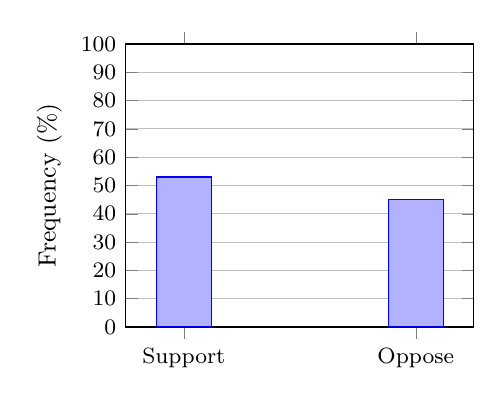
\begin{tikzpicture}
\begin{axis}[
small,
ybar,
width=6cm,
bar width=20pt,
enlarge x limits=0.25,
enlarge y limits=false,
legend style={at={(0.5,-0.2)},
anchor=north,legend columns=-1},
ylabel={Frequency (\%)},
ymajorgrids=true,
symbolic x coords={Support, Oppose},
xtick=data,
%x tick label style={rotate=40,anchor=east},
ytick={0,10,...,100},
ymin=0,
ymax=100,
]
\addplot coordinates {
(Support, 53)
(Oppose, 45)
};
\end{axis}
\end{tikzpicture}
\hskip 1pt
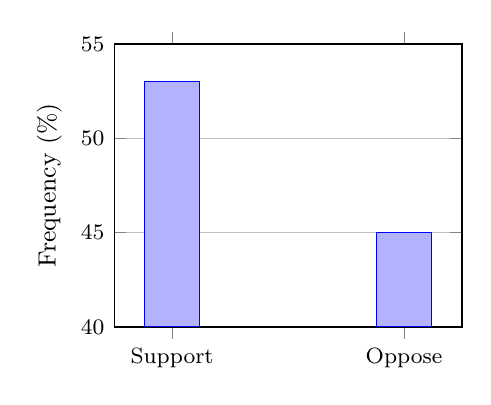
\begin{tikzpicture}
\begin{axis}[
small,
ybar,
width=6cm,
bar width=20pt,
enlarge x limits=0.25,
enlarge y limits=false,
legend style={at={(0.5,-0.2)},
anchor=north,legend columns=-1},
ylabel={Frequency (\%)},
ymajorgrids=true,
symbolic x coords={Support, Oppose},
xtick=data,
%x tick label style={rotate=40,anchor=east},
ytick={0,5,...,100},
ymin=40,
ymax=55,
]
\addplot coordinates {
(Support, 53)
(Oppose, 45)
};
\end{axis}
\end{tikzpicture}

The difference in the vertical scale on the first graph suggests a different story than the true differences in percentages; the second graph makes it look like more than twice as many people support marriage rights as oppose it.
\end{example}
\end{frame}

\begin{frame}
\begin{block}{Definition}
A \textbf{histogram} a bar graph, where the horizontal axis is a number line.
\end{block}\pause

\begin{block}{Definition}
\textbf{Class intervals} are groupings of the data. In general, we define class intervals so that:
\begin{itemize}
\item Each interval is equal size. For example, if the first class contains values from 120-129, then the second class should include 130-139.
\item We have somewhere between 5 and 20 classes, typically, depending upon the number of data we are working with.
\end{itemize}
\end{block}
\end{frame}

\begin{frame}
\begin{example}
A teacher records scores on a 20-point quiz for the 30 students in his class.

\vspace{-6mm}
\begin{center}
\begin{tabular}{lllllllllllllll}
19 & 20 & 18 & 18 & 17 & 18 & 19 & 17 & 20 & 18 & 20 & 16 & 20 & 15 & 17 \\
12 & 18 & 19 & 18 & 19 & 17 & 20 & 18 & 16 & 15 & 18 & 20 &  5 &  0 &  0
\end{tabular}
\end{center}

\vspace{-3mm}
These scores could be summarized in the following histogram.
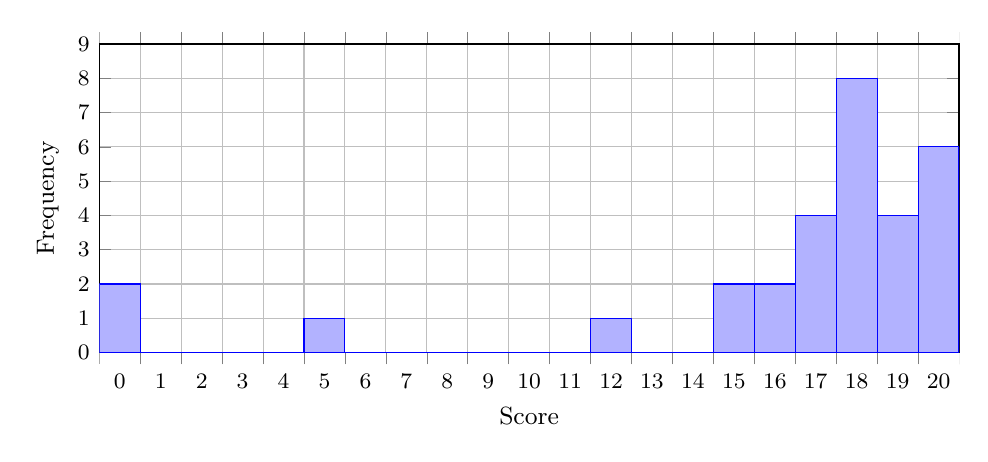
\begin{tikzpicture}
\begin{axis}[
small,
height=5.5cm,
width=12.5cm,
enlarge x limits=false,
enlarge y limits=false,
ybar interval,
ymajorgrids=true,
ylabel={Frequency},
xlabel={Score},
xtick={0,1,...,30},
ytick={0,1,...,30},
ymin=0,
ymax=9,
xmin=0,
xmax=21,
%xticklabel=
%\pgfmathprintnumber\tick--\pgfmathprintnumber\nexttick
]
\addplot+ [hist={bins=21}]
table [row sep=\\,y index=0] {
data\\
19\\ 20\\ 18\\ 18\\ 17\\ 18\\ 19\\ 17\\ 20\\ 18\\ 20\\ 16\\ 20\\ 15\\ 17\\ 12\\ 18\\ 19\\ 18\\ 19\\ 17\\ 20\\ 18\\ 16\\ 15\\ 18\\ 20\\  5\\  0\\  0\\
};
\end{axis}
\end{tikzpicture}
\end{example}
\end{frame}

\begin{frame}
\begin{example}
Suppose that we have collected weights from 100 male subjects as part of a nutrition study. For our weight data, we have values ranging from a low of 121 pounds to a high of 263 pounds, giving a total span of 263-121 = 142.

\vspace{2mm}
\only<1>{%
We could create 6 intervals with a width of around 20.
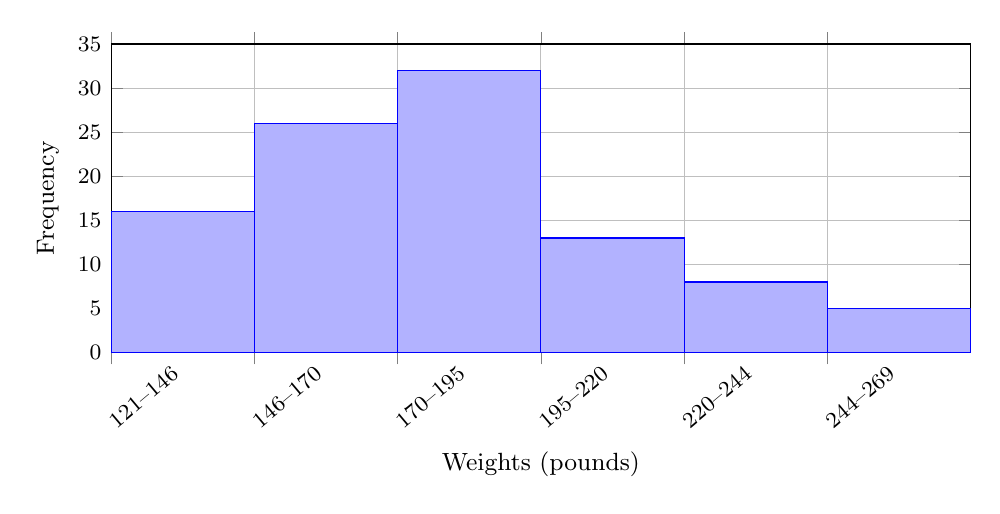
\begin{tikzpicture}
\begin{axis}[
small,
height=5.5cm,
width=12.5cm,
enlarge x limits=false,
enlarge y limits=false,
ybar interval,
ymajorgrids=true,
ylabel={Frequency},
xlabel={Weights (pounds)},
x tick label style={rotate=40,anchor=east},
%xtick={120,140,...,1000},
ytick={0,5,...,1000},
ymin=0,
ymax=35,
%xmin=120,
%xmax=280,
xticklabel style={/pgf/number format/.cd,fixed,precision=0},
xticklabel=
\pgfmathprintnumber\tick--\pgfmathprintnumber\nexttick
]
\addplot+ [hist={bins=6}]
table [row sep=\\,y index=0] {
data\\
121\\ 131\\ 131\\ 130\\ 138\\ 144\\ 147\\ 142\\ 136\\ 141\\ 141\\ 140\\ 138\\ 138\\ 136\\ 140\\ 148\\ 145\\ 153\\ 157\\ 161\\ 155\\ 160\\ 156\\ 157\\ 155\\ 156\\ 161\\ 150\\ 156\\ 160\\ 157\\ 151\\ 155\\ 174\\ 175\\ 171\\ 168\\ 176\\ 168\\ 174\\ 176\\ 176\\ 172\\ 175\\ 172\\ 176\\ 166\\ 175\\ 176\\ 168\\ 175\\ 168\\ 178\\ 178\\ 169\\ 169\\ 170\\ 172\\ 178\\ 171\\ 173\\ 181\\ 183\\ 186\\ 189\\ 188\\ 180\\ 187\\ 192\\ 185\\ 188\\ 188\\ 182\\ 207\\ 203\\ 207\\ 207\\ 205\\ 208\\ 208\\ 204\\ 216\\ 214\\ 216\\ 221\\ 211\\ 212\\ 223\\ 236\\ 230\\ 226\\ 232\\ 225\\ 230\\ 248\\ 245\\ 265\\ 267\\ 269\\
};
\end{axis}
\end{tikzpicture} 
}\only<2>{%
We could create 8 intervals with a width of around 18.
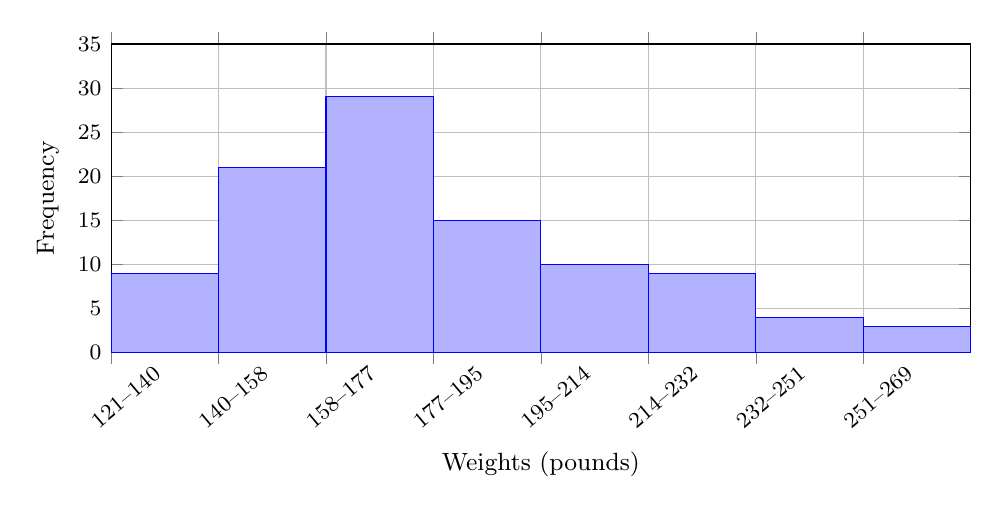
\begin{tikzpicture}
\begin{axis}[
small,
height=5.5cm,
width=12.5cm,
enlarge x limits=false,
enlarge y limits=false,
ybar interval,
ymajorgrids=true,
ylabel={Frequency},
xlabel={Weights (pounds)},
x tick label style={rotate=40,anchor=east},
%xtick={120,140,...,1000},
ytick={0,5,...,1000},
ymin=0,
ymax=35,
%xmin=120,
%xmax=280,
xticklabel style={/pgf/number format/.cd,fixed,precision=0},
xticklabel=
\pgfmathprintnumber\tick--\pgfmathprintnumber\nexttick
]
\addplot+ [hist={bins=8}]
table [row sep=\\,y index=0] {
data\\
121\\ 131\\ 131\\ 130\\ 138\\ 144\\ 147\\ 142\\ 136\\ 141\\ 141\\ 140\\ 138\\ 138\\ 136\\ 140\\ 148\\ 145\\ 153\\ 157\\ 161\\ 155\\ 160\\ 156\\ 157\\ 155\\ 156\\ 161\\ 150\\ 156\\ 160\\ 157\\ 151\\ 155\\ 174\\ 175\\ 171\\ 168\\ 176\\ 168\\ 174\\ 176\\ 176\\ 172\\ 175\\ 172\\ 176\\ 166\\ 175\\ 176\\ 168\\ 175\\ 168\\ 178\\ 178\\ 169\\ 169\\ 170\\ 172\\ 178\\ 171\\ 173\\ 181\\ 183\\ 186\\ 189\\ 188\\ 180\\ 187\\ 192\\ 185\\ 188\\ 188\\ 182\\ 207\\ 203\\ 207\\ 207\\ 205\\ 208\\ 208\\ 204\\ 216\\ 214\\ 216\\ 221\\ 211\\ 212\\ 223\\ 236\\ 230\\ 226\\ 232\\ 225\\ 230\\ 248\\ 245\\ 265\\ 267\\ 269\\
};
\end{axis}
\end{tikzpicture} 
}\only<3>{%
We could create 10 intervals with a width of around 14.
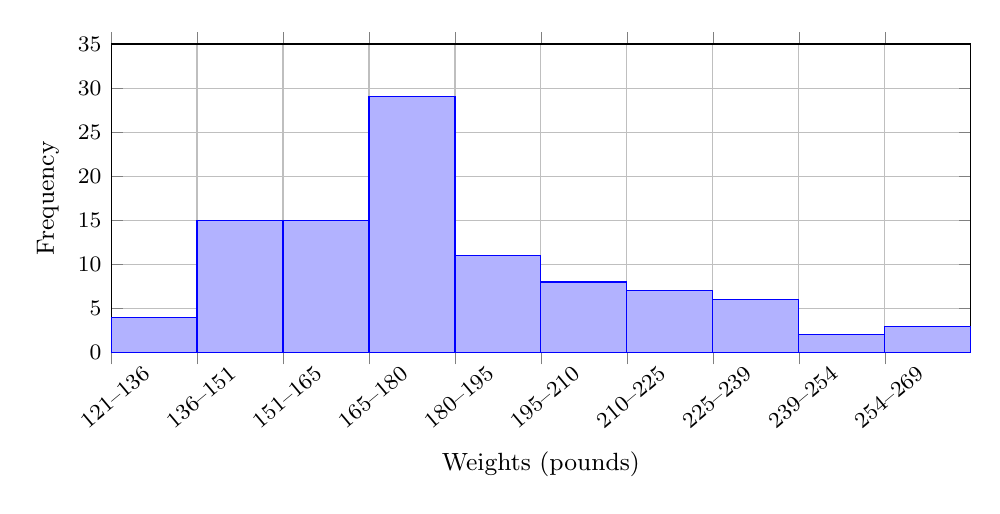
\begin{tikzpicture}
\begin{axis}[
small,
height=5.5cm,
width=12.5cm,
enlarge x limits=false,
enlarge y limits=false,
ybar interval,
ymajorgrids=true,
ylabel={Frequency},
xlabel={Weights (pounds)},
x tick label style={rotate=40,anchor=east},
%xtick={120,140,...,1000},
ytick={0,5,...,1000},
ymin=0,
ymax=35,
%xmin=120,
%xmax=280,
xticklabel style={/pgf/number format/.cd,fixed,precision=0},
xticklabel=
\pgfmathprintnumber\tick--\pgfmathprintnumber\nexttick
]
\addplot+ [hist={bins=10}]
table [row sep=\\,y index=0] {
data\\
121\\ 131\\ 131\\ 130\\ 138\\ 144\\ 147\\ 142\\ 136\\ 141\\ 141\\ 140\\ 138\\ 138\\ 136\\ 140\\ 148\\ 145\\ 153\\ 157\\ 161\\ 155\\ 160\\ 156\\ 157\\ 155\\ 156\\ 161\\ 150\\ 156\\ 160\\ 157\\ 151\\ 155\\ 174\\ 175\\ 171\\ 168\\ 176\\ 168\\ 174\\ 176\\ 176\\ 172\\ 175\\ 172\\ 176\\ 166\\ 175\\ 176\\ 168\\ 175\\ 168\\ 178\\ 178\\ 169\\ 169\\ 170\\ 172\\ 178\\ 171\\ 173\\ 181\\ 183\\ 186\\ 189\\ 188\\ 180\\ 187\\ 192\\ 185\\ 188\\ 188\\ 182\\ 207\\ 203\\ 207\\ 207\\ 205\\ 208\\ 208\\ 204\\ 216\\ 214\\ 216\\ 221\\ 211\\ 212\\ 223\\ 236\\ 230\\ 226\\ 232\\ 225\\ 230\\ 248\\ 245\\ 265\\ 267\\ 269\\
};
\end{axis}
\end{tikzpicture} 
}\only<4>{%
We could create 10 intervals with a width of around 12.
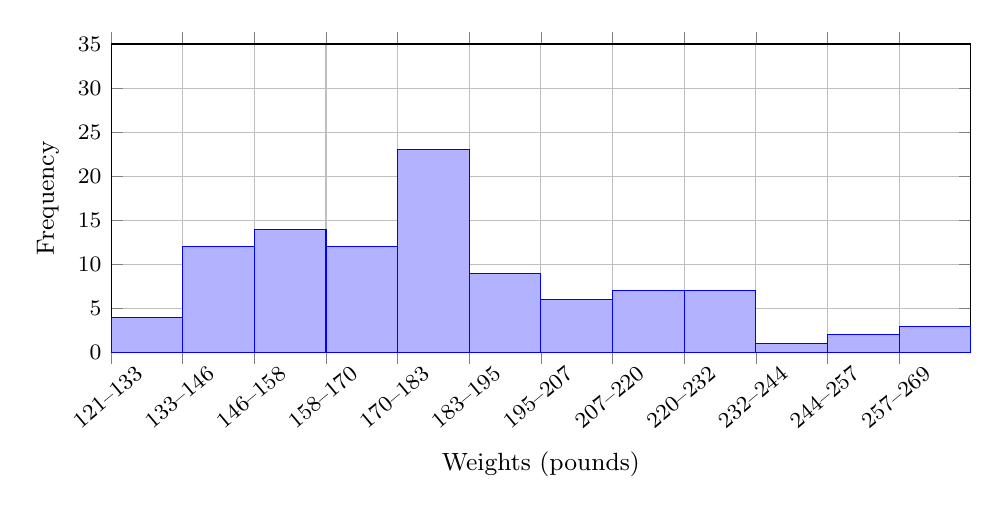
\begin{tikzpicture}
\begin{axis}[
small,
height=5.5cm,
width=12.5cm,
enlarge x limits=false,
enlarge y limits=false,
ybar interval,
ymajorgrids=true,
ylabel={Frequency},
xlabel={Weights (pounds)},
x tick label style={rotate=40,anchor=east},
%xtick={120,140,...,1000},
ytick={0,5,...,1000},
ymin=0,
ymax=35,
%xmin=120,
%xmax=280,
xticklabel style={/pgf/number format/.cd,fixed,precision=0},
xticklabel=
\pgfmathprintnumber\tick--\pgfmathprintnumber\nexttick
]
\addplot+ [hist={bins=12}]
table [row sep=\\,y index=0] {
data\\
121\\ 131\\ 131\\ 130\\ 138\\ 144\\ 147\\ 142\\ 136\\ 141\\ 141\\ 140\\ 138\\ 138\\ 136\\ 140\\ 148\\ 145\\ 153\\ 157\\ 161\\ 155\\ 160\\ 156\\ 157\\ 155\\ 156\\ 161\\ 150\\ 156\\ 160\\ 157\\ 151\\ 155\\ 174\\ 175\\ 171\\ 168\\ 176\\ 168\\ 174\\ 176\\ 176\\ 172\\ 175\\ 172\\ 176\\ 166\\ 175\\ 176\\ 168\\ 175\\ 168\\ 178\\ 178\\ 169\\ 169\\ 170\\ 172\\ 178\\ 171\\ 173\\ 181\\ 183\\ 186\\ 189\\ 188\\ 180\\ 187\\ 192\\ 185\\ 188\\ 188\\ 182\\ 207\\ 203\\ 207\\ 207\\ 205\\ 208\\ 208\\ 204\\ 216\\ 214\\ 216\\ 221\\ 211\\ 212\\ 223\\ 236\\ 230\\ 226\\ 232\\ 225\\ 230\\ 248\\ 245\\ 265\\ 267\\ 269\\
};
\end{axis}
\end{tikzpicture}
}\only<5>{%
We could create 14 intervals with a width of around 10.
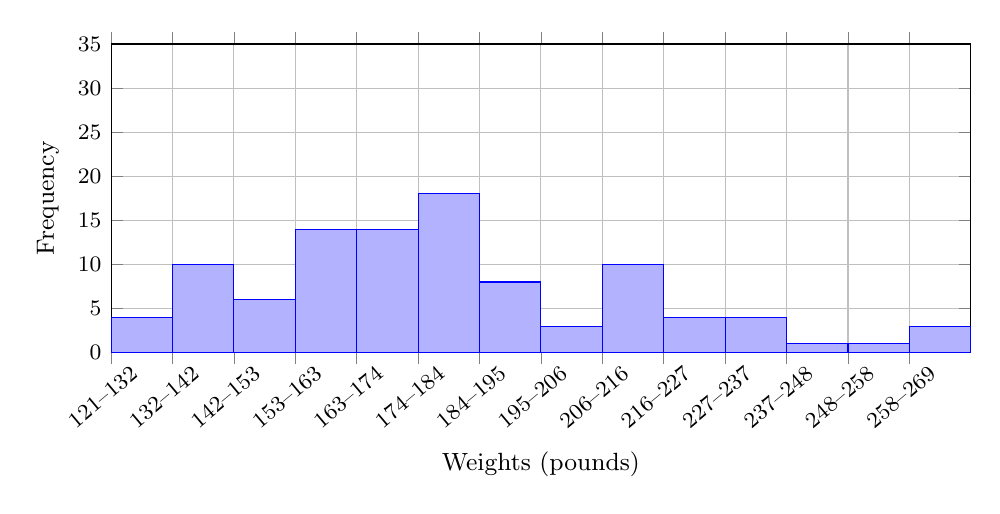
\begin{tikzpicture}
\begin{axis}[
small,
height=5.5cm,
width=12.5cm,
enlarge x limits=false,
enlarge y limits=false,
ybar interval,
ymajorgrids=true,
ylabel={Frequency},
xlabel={Weights (pounds)},
x tick label style={rotate=40,anchor=east},
%xtick={120,140,...,1000},
ytick={0,5,...,1000},
ymin=0,
ymax=35,
%xmin=120,
%xmax=280,
xticklabel style={/pgf/number format/.cd,fixed,precision=0},
xticklabel=
\pgfmathprintnumber\tick--\pgfmathprintnumber\nexttick
]
\addplot+ [hist={bins=14}]
table [row sep=\\,y index=0] {
data\\
121\\ 131\\ 131\\ 130\\ 138\\ 144\\ 147\\ 142\\ 136\\ 141\\ 141\\ 140\\ 138\\ 138\\ 136\\ 140\\ 148\\ 145\\ 153\\ 157\\ 161\\ 155\\ 160\\ 156\\ 157\\ 155\\ 156\\ 161\\ 150\\ 156\\ 160\\ 157\\ 151\\ 155\\ 174\\ 175\\ 171\\ 168\\ 176\\ 168\\ 174\\ 176\\ 176\\ 172\\ 175\\ 172\\ 176\\ 166\\ 175\\ 176\\ 168\\ 175\\ 168\\ 178\\ 178\\ 169\\ 169\\ 170\\ 172\\ 178\\ 171\\ 173\\ 181\\ 183\\ 186\\ 189\\ 188\\ 180\\ 187\\ 192\\ 185\\ 188\\ 188\\ 182\\ 207\\ 203\\ 207\\ 207\\ 205\\ 208\\ 208\\ 204\\ 216\\ 214\\ 216\\ 221\\ 211\\ 212\\ 223\\ 236\\ 230\\ 226\\ 232\\ 225\\ 230\\ 248\\ 245\\ 265\\ 267\\ 269\\
};
\end{axis}
\end{tikzpicture}
}
\vspace{-5mm}
\end{example}
\end{frame}

\begin{frame}
\begin{block}{Definition}
The \textbf{mean} of a set of data is the sum of the data values divided by the number of values.
\end{block}\pause

\begin{block}{Note}
It is not uncommon to see the word \textquote{average} used instead of \textquote{mean}.
\end{block}\pause

\begin{example}
Marci's exam scores for her last math class were: 79, 86, 82, 94. 

What is the mean of these values?\pause
\begin{equation*}
\dfrac{79+86+82+94}{4}=\dfrac{341}{4}=82.25\approx 85.3
\end{equation*}
Typically we round means to one more decimal than the original data.
\end{example}\pause
\end{frame}

\begin{frame}
\begin{example}
The one hundred families in a particular neighborhood are asked their annual household income, to the nearest \$5 thousand dollars. 
\begin{center}
\begin{tabular}{|c|c||c|c|}
\hline
Income & Frequency & Income & Frequency \\\hline
15 &6 & 35 &19\\\hline
20 &8 & 40 &20\\\hline
25 &11 & 45 &12\\\hline
30 &17 & 50 &7\\\hline
\end{tabular}
\end{center}
What is the mean of this data?\pause
\begin{equation*}
\begin{aligned}
&\dfrac{\overbrace{15+\cdots+15}^{\text{6 terms}}+\overbrace{20+\cdots+20}^{\text{8 terms}}+\overbrace{25+\cdots+25}^{\text{11 terms}}+\cdots+\overbrace{50+\cdots+25}^{\text{7 terms}}}{100} \\
=&\dfrac{15\cdot 6+20\cdot 8+25\cdot 11+30\cdot 17+35\cdot 19+40\cdot 20+45\cdot 12+50\cdot 7}{100} \\
=& \dfrac{3390}{100} = 33.9
\end{aligned}
\end{equation*}
\end{example}
\end{frame}

\begin{frame}
\begin{block}{Definition}
The \textbf{median} of a set of data is the value in the middle when the data is in numerical order.
\end{block}\pause

\begin{block}{Note}
To find the median, begin by listing the data in order from smallest to largest, or largest to smallest.

\vspace{2mm}
If the number of data values, $N$, is odd, then the median is the middle data value. This value can be found by rounding $\frac{N}{2}$ up to the next whole number.

\vspace{2mm}
If the number of data values is even, there is no one middle value, so we find the mean
of the two middle values (values $\frac{N}{2}$ and $\frac{N}{2} + 1$)
\end{block}
\end{frame}

\begin{frame}
\begin{example}
Find the media of these quiz scores: 8 6 4 1 7 1 1\pause

\vspace{2mm}
List the data in order: 1 1 1 $\underset{\Uparrow}{4}$ 6 7 8

\vspace{2mm}
Since we have an odd number of data, we see the median is 4.
\end{example}\pause

\begin{example}
Find the median of these quiz scores: 5 9 8 6 4 8 2 5 7 7\pause

\vspace{2mm}
List the data in order: 2 4 5 5 6 $\underset{\Uparrow}{}$ 7 7 8 8 9

\vspace{2mm}
Since we have an even number of data, there is no middle item. In this case, we say the median is the mean of the two middle numbers, 6 and 7, which is 6.5.
\end{example}
\end{frame}

\begin{frame}
\begin{example}
The one hundred families in a particular neighborhood are asked their annual household income, to the nearest \$5 thousand dollars. 

\vspace{-3mm}
\begin{center}
\begin{tabular}{|c|c||c|c|}
\hline
Income & Frequency & Income & Frequency \\\hline
15 &6 & 35 &19\\\hline
20 &8 & 40 &20\\\hline
25 &11 & 45 &12\\\hline
30 &17 & 50 &7\\\hline
\end{tabular}
\end{center}

\vspace{-3mm}
What is the median of this data?\pause

\vspace{1mm}
We have 100 items, this means the median will be the mean of the $50^{\small\text{th}}$ and $51^{\small\text{st}}$ data values. So, we need to start counting up from the bottom:\pause
\vspace{-6mm}
\begin{center}
\begin{tabular}{lcl}
There are 6 data values of 15. & $\Rightarrow$ & Values 1 to 6 are 15. \\\pause
The next 8 data values are 20. & $\Rightarrow$ & Values 7 to (6+8)=14 are 20. \\\pause
The next 11 data values are 25. & $\Rightarrow$ & Values 15 to (14+11)=25 are 25. \\\pause
The next 17 data values are 30. & $\Rightarrow$ & Values 26 to (25+17)=42 are 30. \\\pause
The next 19 data values are 35. & $\Rightarrow$ & Values 43 to (42+19)=61 are 35.
\end{tabular}
\end{center}\pause

\vspace{-2mm}
So, the median is $\frac{35+35}{2}=35$, \$35 thousand dollars.
\end{example}
\end{frame}

\begin{frame}
\begin{block}{Definition}
The \textbf{mode} is the element of the data set that occurs most frequently.
\end{block}\pause

\begin{block}{Note}
The mode is useless with quantitative data. It is most commonly used for categorical data, for which median and mean cannot be computed. 
\end{block}\pause

\begin{example}
In Example~\ref{ex:carcolor1} we collected the data:

\vspace{-2mm}
\begin{center}
\begin{tabular}{|c|c||c|c|}
\hline
Color & Frequency & Color & Frequency \\\hline
Blue & 3 & White & 3\\\hline
Green & 5 & Black & 2\\\hline
Red & 4 & Grey & 3\\\hline
\end{tabular}
\end{center}

\vspace{-2mm}
For this data, Green is the mode.
\end{example}\pause

\begin{block}{Note}
It is possible for a data set to have more than one mode.
\end{block}
\end{frame}
\end{document}
